%beamer

% TODO:
% - VL-Folien einarbeiten
% - Weniger f_* etc. Theorie, mehr Aufgaben zwischendrin und zu Akzeptoren
% - Bessere Hinleitung zu Akzeptoren

% Comment/uncomment this line to toggle handout mode
\newcommand{\handout}{}

%% Beamer-Klasse im korrekten Modus
\ifdefined \handout
\documentclass[handout]{beamer} % Handout mode
\else
\documentclass{beamer}
\fi

%% UTF-8-Encoding
\usepackage[utf8]{inputenc}

\input{../framework/gbi-macros}
\usepackage[blue]{../framework/thwregex}
\usepackage{environ}
\usepackage{bm}
\usepackage{calc}
\usepackage{varwidth}
\usepackage{wasysym}
\usepackage{mathtools}


% Das ist der KIT-Stil
%\usepackage{../TutTexbib/beamerthemekit}
\usepackage[deutsch,titlepage0]{../framework/KIT/beamerthemeKITmod}
\TitleImage[width=\titleimagewd]{../figures/titlepage.jpg}
%\usetheme[deutsch,titlepage0]{KIT}

% Include PDFs
\usepackage{pdfpages}

% Libertine font (Original GBI font)
\usepackage{libertine}
%\renewcommand*\familydefault{\sfdefault}  %% Only if the base font of the document is to be sans serif

% Nicer math symbols
\usepackage{eulervm}
%\usepackage{mathpazo}
\renewcommand\ttdefault{cmtt} % Computer Modern typewriter font, see lecture slides.

\usepackage{csquotes}

%%%%%%

%% Schönere Schriften
\usepackage[TS1,T1]{fontenc}

%% Bibliothek für Graphiken
\usepackage{graphicx}

%% der wird sowieso in jeder Datei gesetzt
\graphicspath{{../figures/}}

%% Anzeigetiefe für Inhaltsverzeichnis: 1 Stufe
\setcounter{tocdepth}{1}

%% Hyperlinks
\usepackage{hyperref}
% I don't know why, but this works and only includes sections and NOT subsections in the pdf-bookmarks.
\hypersetup{bookmarksdepth=subsection} 

%\usepackage{lmodern}
\usepackage{colortbl}
\usepackage[absolute,overlay]{textpos}
\usepackage{listings}
\usepackage{forloop}
%\usepackage{algorithmic} % PseudoCode package 

\usepackage{tikz}
\usetikzlibrary{matrix}
\usetikzlibrary{arrows.meta}
\usetikzlibrary{automata}
\usetikzlibrary{tikzmark}
\usetikzlibrary{positioning}

% Why has no-one come up with this yet? I mean, seriously. -.-
\tikzstyle{loop below right} = [loop, out=-60,in=-30, looseness=7]
\tikzstyle{loop below left} = [loop, out=-150,in=-120, looseness=7]
\tikzstyle{loop above right} = [loop, out=60,in=30, looseness=7]
\tikzstyle{loop above left} = [loop, out=150,in=120, looseness=7]
\tikzstyle{loop right below} = [loop below right]
\tikzstyle{loop left below} = [loop below left]
\tikzstyle{loop right above} = [loop above right]
\tikzstyle{loop left above} = [loop above left]

% Needed for gbi-macros
\usepackage{xspace}

%%%%%%

%% Verbatim
\usepackage{moreverb}

%%%%%%%%%%%%%%%%%%%%%%%%%%%%%%%%%%%% Copy end

%% Tabellen
\usepackage{array}
\usepackage{multicol}
\usepackage{hhline}

%% Bibliotheken für viele mathematische Symbole
\usepackage{amsmath, amsfonts, amssymb}

%% Deutsche Silbentrennung und Beschriftungen
\usepackage[ngerman]{babel}

\usepackage{kbordermatrix}

% kbordermatrix settings
\renewcommand{\kbldelim}{(} % Left delimiter
\renewcommand{\kbrdelim}{)} % Right delimiter

\input{../config.tex}



% define custom \handout command flag if handout mode is toggled  #DirtyAsHellButWell...
\only<beamer:0>{\def\handout{}} %beamer:0 == handout mode

\newcommand{\R}{\mathbb{R}}
\newcommand{\N}{\mathbb{N}}
\newcommand{\Z}{\mathbb{Z}}
\newcommand{\Q}{\mathbb{Q}}
\newcommand{\BB}{\mathbb{B}}
\newcommand{\C}{\mathbb{C}}
\newcommand{\K}{\mathbb{K}}
\newcommand{\G}{\mathbb{G}}
\newcommand{\nullel}{\mathcal{O}}
\newcommand{\einsel}{\mathds{1}}
\newcommand{\Pot}{\mathcal{P}}
\renewcommand{\O}{\text{O}}

\def\word#1{\hbox{\textcolor{blue}{\texttt{#1}}}}
\let\literal\word
\def\mword#1{\hbox{\textcolor{blue}{$\mathtt{#1}$}}}  % math word
\def\sp{\scalebox{1}[.5]{\textvisiblespace}}
\def\wordsp{\word{\sp}}

%\newcommand{\literal}[1]{\textcolor{blue}{\texttt{#1}}}
\newcommand{\realTilde}{\textasciitilde \ }
\newcommand{\setsize}[1]{\ensuremath{\left\lvert #1 \right\rvert}}
\newcommand{\size}[1]{\setsize{#1}}  % Shame on you, TeXStudio...
\newcommand{\set}[1]{\left\{#1\right\}}
\newcommand{\tuple}[1]{\left(#1\right)}
\newcommand{\normalvar}[1]{\text{$#1$}}

% Modified by DJ
\let\oldemptyset\emptyset
\let\emptyset\varnothing % proper emptyset

\newcommand{\boder}{\ensuremath{\mathbin{\textcolor{blue}{\vee}}}\xspace}
\newcommand{\bund}{\ensuremath{\mathbin{\textcolor{blue}{\wedge}}}\xspace}
\newcommand{\bimp}{\ensuremath{\mathrel{\textcolor{blue}{\to}}}\xspace}
\newcommand{\bgdw}{\ensuremath{\mathrel{\textcolor{blue}{\leftrightarrow}}}\xspace}
\newcommand{\bnot}{\ensuremath{\textcolor{blue}{\neg}}\xspace}
\newcommand{\bone}{\ensuremath{\textcolor{blue}{1}}\text{}}
\newcommand{\bzero}{\ensuremath{\textcolor{blue}{0}}\text{}}
\newcommand{\bleftBr}{\ensuremath{\textcolor{blue}{\texttt{(}}}\text{}}
\newcommand{\brightBr}{\ensuremath{\textcolor{blue}{\texttt{)}}}\text{}}

% Fix of \b... commands:

\renewcommand{\boder}{\alor}
\renewcommand{\bund}{\aland}
\renewcommand{\bimp}{\alimpl}
\renewcommand{\bgdw}{\aleqv}
\renewcommand{\bnot}{\alnot}
\renewcommand{\bleftBr}{\alka}
\renewcommand{\brightBr}{\alkz}
\newcommand{\alA}{\word A}
\newcommand{\alB}{\word B}
\newcommand{\alC}{\word C}

\newcommand{\plB}{\plfoo{B}}
\newcommand{\plE}{\plfoo{E}}

\newcommand{\summe}[2]{\sum\limits_{#1}^{#2}}
\newcommand{\limes}[1]{\lim\limits_{#1}}

%\newcommand{\numpp}{\advance \value{weeknum} by -2 \theweeknum \advance \value{weeknum} by 2}
%\newcommand{\nump}{\advance \value{weeknum} by -1 \theweeknum \advance \value{weeknum} by 1}

\newcommand{\mycomment}[1]{}
\newcommand{\Comment}[1]{}

%% DISCLAIMER START 
% It is INSANELY IMPORTANT NOT TO DO THIS OUTSIDE BEAMER CLASS! IN ARTCILE DOCUMENTS, THIS IS VERY LIKELY TO BUG AROUND!
\makeatletter%
\@ifclassloaded{beamer}%
{
	% TODO 
	% no time... later.   (= never -.-)
	% redefine section to ignore multiple \section calls with the same title
}%
{
	\errmessage{ERROR: section command redefinition outside of beamer class document! Please contact the author of this code or read the F-ing disclaimer.}
}%
\makeatother%
%% DISCLAIMER END

\newcounter{abc}
\newenvironment{alist}{
  \begin{list}{(\alph{abc})}{
      \usecounter{abc}\setlength{\leftmargin}{8mm}\setlength{\labelsep}{2mm}
    }
}{\end{list}}


\newcommand{\stdarraystretch}{1.20}
\renewcommand{\arraystretch}{\stdarraystretch}  % for proper row spacing in tables

\newcommand{\morescalingdelimiters}{   % for proper \left( \right) typography
	\delimitershortfall=-1pt  
	\delimiterfactor=1
}

\newcommand{\centered}[1]{\vspace{-\baselineskip}\begin{center}#1\end{center}\vspace{-\baselineskip}}

% for \implitem and \item[bla] stuff to look right:
\setbeamercolor*{itemize item}{fg=black}
\setbeamercolor*{itemize subitem}{fg=black}
\setbeamercolor*{itemize subsubitem}{fg=black}

\setbeamercolor*{description item}{fg=black}
\setbeamercolor*{description subitem}{fg=black}
\setbeamercolor*{description subsubitem}{fg=black}

\renewcommand{\qedsymbol}{\textcolor{black}{\openbox}}

\renewcommand{\mod}{\mathop{\textbf{mod}}}
\renewcommand{\div}{\mathop{\textbf{div}}}

\newcommand{\ceil}[1]{\left\lceil#1\right\rceil}
\newcommand{\floor}[1]{\left\lfloor#1\right\rfloor}
\newcommand{\abs}[1]{\left\lvert #1 \right\rvert}
\newcommand{\Matrix}[1]{\begin{pmatrix} #1 \end{pmatrix}}
\newcommand{\braced}[1]{\left\lbrace #1 \right\rbrace}

% "something" placeholder. Useful for repairing spacing of operator sections, like `\sth = 42`.
\def\sth{\vphantom{.}}

\def\fract#1/#2 {\frac{#1}{#2}} % ! Trailing space is crucial!
\def\dfract#1/#2 {\dfrac{#1}{#2}} % ! Trailing space is crucial!

\newcommand{\Mid}{\;\middle|\;}

\let\after\circ



\def\·{\cdot}
\def\*{\cdot}
\def\?>{\ensuremath{\rightsquigarrow}}  % Fuck you, Latex
\def\~~>{\ensuremath{\rightsquigarrow}}  

\newcommand{\tight}[1]{{\renewcommand{\arraystretch}{0.76} #1}}
\newcommand{\stackedtight}[1]{\renewcommand{\arraystretch}{0.76} \begin{matrix} #1 \end{matrix} }
\newcommand{\stacked}[1]{\begin{matrix} #1 \end{matrix} }
\newcommand{\casesl}[1]{\delimitershortfall=0pt  \left\lbrace\hspace{-.3\baselineskip}\begin{array}{ll} #1 \end{array}\right.}
\newcommand{\casesr}[1]{\delimitershortfall=0pt  \left.\begin{array}{ll} #1 \end{array}\hspace{-.3\baselineskip}\right\rbrace}
\newcommand{\caseslr}[1]{\delimitershortfall=0pt  \left\lbrace\hspace{-.3\baselineskip}\begin{array}{ll} #1 \end{array}\hspace{-.3\baselineskip}\right\rbrace}

\def\q#1uad{\ifnum#1=0\relax\else\quad\q{\the\numexpr#1-1\relax}uad\fi}
% e.g. \q1uad = \quad, \q2uad = \qquad etc.

\newcommand{\qqquad}{\q3uad}
\newcommand{\minusquad}{\hspace{-1em}}

%% Placeholder utils
% \§{#1}   Saves #1 as placeholder and prints it
% \.       Prints an \hphantom with the size of the recalled placeholder.
\def\indentstring{}
\def\§#1{\def\indentstring{#1}#1}
\def\.{{$\hphantom{\text{\indentstring}}$}}
%% Placeholder utils end

\newcommand{\impl}{\ifmmode\ensuremath{\mskip\thinmuskip\Rightarrow\mskip\thinmuskip}\else$\Rightarrow$\fi\xspace}
\newcommand{\Impl}{\ifmmode\implies\else$\Longrightarrow$\fi\xspace}

\newcommand{\derives}{\Rightarrow}

\newcommand{\gdw}{\ifmmode\mskip\thickmuskip\Leftrightarrow\mskip\thickmuskip\else$\Leftrightarrow$\fi\xspace}
\newcommand{\Gdw}{\ifmmode\iff\else$\Longleftrightarrow$\fi\xspace}

% Legacy code from the algo tutorial slides. Perhaps useful. Try with care.
\mycomment{
	\newcommand{\impl}{\ifmmode\ensuremath{\mskip\thinmuskip\Rightarrow\mskip\thinmuskip}\else$\Rightarrow$\xspace\fi}  
	\newcommand{\Impl}{\ifmmode\implies\else$\Longrightarrow$\xspace\fi}
	
	\newcommand{\gdw}{\ifmmode\mskip\thickmuskip\Leftrightarrow\mskip\thickmuskip\else$\Leftrightarrow$\xspace\fi}
	\newcommand{\Gdw}{\ifmmode\iff\else$\Longleftrightarrow$\xspace\fi}
}
	
\newcommand{\gdwdef}{\ifmmode\mskip\thickmuskip:\Leftrightarrow\mskip\thickmuskip\else:$\Leftrightarrow$\xspace\fi}
\newcommand{\Gdwdef}{\ifmmode\mskip\thickmuskip:\Longleftrightarrow\mskip\thickmuskip\else:$\Longleftrightarrow$\xspace\fi}

\newcommand{\symbitemnegoffset}{\hspace{-.5\baselineskip}}
\newcommand{\implitem}{\item[\impl\symbitemnegoffset]}
\newcommand{\Implitem}{\item[\Impl\symbitemnegoffset]}


\newcommand{\forcenewline}{\mbox{}\\}

\newcommand{\bfalert}[1]{\textbf{\alert{#1}}}
\let\elem\in   % I'm a Haskell freak. Don't judge me. :P


\def\|#1|{\text{\normalfont #1}}  % | steht für senkrecht (anstatt kursiv wie sonst im math mode)


% proper math typography
\newcommand{\functionto}{\longrightarrow}
\renewcommand{\geq}{\geqslant}
\renewcommand{\leq}{\leqslant}
\let\oldsubset\subset
\renewcommand{\subset}{\subseteq} % for all idiots out there using subset

\newenvironment{threealign}{%
	\[
	\begin{array}{r@{\ }c@{\ }l}
}{%
	\end{array}	
	\]
}

\newcommand{\concludes}{ \\ \hline  }
\newcommand{\deduction}[1]{
	\begin{varwidth}{.8\linewidth}
		\begin{tabular}{>{$}c<{$}}
			#1
		\end{tabular}
	\end{varwidth}	
}

\definecolor{hoareorange}{rgb}{1,.85,.6}
\newcommand{\hoareassert}[1]{\setlength{\fboxsep}{1pt}\setlength{\fboxrule}{-1.4pt}\fcolorbox{white}{hoareorange}{\ensuremath{\{\;#1\;\}}}\setlength\fboxrule{\defaultfboxrule}\setlength{\fboxsep}{3pt}}

\newcommand{\mailto}[1]{\href{mailto:#1}{{\textcolor{blue}{\underline{#1}}}}}
\newcommand{\urlnamed}[2]{\href{#2}{\textcolor{blue}{\underline{#1}}}}
\renewcommand{\url}[1]{\urlnamed{#1}{#1}}

\newcommand{\hanging}{\hangindent=0.7cm}
\newcommand{\indented}{\hanging}


% \hstretchto prints #2 left-aligned into a box of the width of #1
\def\hstretchto#1#2{%
	\mbox{}\vphantom{#2}\rlap{#2}\hphantom{#1}%
}

\def\vstretchto#1#2{%
	\mbox{}\hphantom{#2}\smash{#2}\vphantom{#1}%
}

% \hstretchtocentered prints #2 centered into a box of the width of #1
\def\hstretchtocentered#1#2{%
	\mbox{}\vphantom{#2}\scalebox{0.5}{\hphantom{#1}}\clap{#2}\scalebox{0.5}{\hphantom{#1}}%
}

% vertical centering
\newcommand{\vertcenter}[1]{%
	\ensuremath{\vcenter{\hbox{#1}}}%
}


%requires \thisyear to be defined (s. config.tex)!
\edef\nextyear{\the\numexpr\thisyear+1\relax}


% --- \frameheight constant ---
\newlength\fullframeheight
\newlength\framewithtitleheight
\setlength\fullframeheight{.92\textheight}
\setlength\framewithtitleheight{.86\textheight}

\newlength\frameheight
\setlength\frameheight{\fullframeheight}

\let\frametitleentry\relax
\let\oldframetitle\frametitle
\def\newframetitle#1{\global\def\frametitleentry{#1}\if\relax\frametitleentry\relax\else\setlength\frameheight{\framewithtitleheight}\fi\oldframetitle{#1}}
\let\frametitle\newframetitle

\def\newframetitleoff{\let\frametitle\oldframetitle}
\def\newframetitleon{\let\frametitle\newframetitle}
% --- \frameheight constant end ---

\newcommand{\fakeframetitle}[1]{%
	\vspace{-2.05\baselineskip}%
	{\Large \textbf{#1}} \\%
	\smallskip
}



\newenvironment{headframe}{\Huge THIS IS AN ERROR. PLEASE CONTACT THE ADMIN OF THIS TEX CODE. (headframe env def failed)}{}
\RenewEnviron{headframe}[1][]{
	\begin{frame}\frametitle{\ }
		\centering
		\Huge\textbf{\textsc{\BODY} \\
		}
		\Large {#1}
		\frametitle{\ }
	\end{frame}
}


\makeatletter
% Provides color if undefined.
\newcommand{\colorprovide}[2]{%
	\@ifundefinedcolor{#1}{\colorlet{#1}{#2}}{}}
\makeatother


\colorprovide{lightred}{red!30}
\colorprovide{lightgreen}{green!40}
\colorprovide{lightyellow}{yellow!50}
\colorprovide{lightblue}{blue!10}
\colorprovide{beamerlightred}{lightred}
\colorprovide{beamerlightgreen}{lightgreen}
\colorprovide{beamerlightyellow}{lightyellow}
\colorprovide{beamerlightblue}{lightblue}
\colorprovide{fullred}{red!60}
\colorprovide{fullgreen}{green}
\definecolor{darkred}{RGB}{115,48,38}
\definecolor{darkgreen}{RGB}{48,115,38}
\definecolor{darkyellow}{RGB}{100,100,0}

\only<handout:0>{\colorlet{adaptinglightred}{beamerlightred}}
\only<handout:0>{\colorlet{adaptinglightgreen}{beamerlightgreen}}
\only<handout:0>{\colorlet{adaptinglightyellow}{beamerlightyellow}}
\only<handout:0>{\colorlet{adaptinglightblue}{beamerlightblue}}
\only<beamer:0>{\colorlet{adaptinglightred}{lightred}}
\only<beamer:0>{\colorlet{adaptinglightgreen}{lightgreen}}
\only<beamer:0>{\colorlet{adaptinglightyellow}{lightyellow}}
\only<beamer:0>{\colorlet{adaptinglightblue}{lightblue}}
\only<handout:0>{\colorlet{adaptingred}{lightred}}
\only<beamer:0>{\colorlet{adaptingred}{fullred}}
\only<handout:0>{\colorlet{adaptinggreen}{lightgreen}}
\only<beamer:0>{\colorlet{adaptinggreen}{fullgreen}}



\newcommand{\TrueQuestion}[1]{
	\TrueQuestionE{#1}{}
}

\newcommand{\YesQuestion}[1]{
	\YesQuestionE{#1}{}
}

\newcommand{\FalseQuestion}[1]{
	\FalseQuestionE{#1}{}
}

\newcommand{\NoQuestion}[1]{
	\NoQuestionE{#1}{}
}

\newcommand{\DependsQuestion}[1]{
	\DependsQuestionE{#1}{}
}

\newcommand{\QuestionVspace}{\vspace{4pt}}
\newcommand{\QuestionParbox}[1]{\begin{varwidth}{.85\linewidth}#1\end{varwidth}}
\newcommand{\ExplanationParbox}[1]{\begin{varwidth}{.97\linewidth}#1\end{varwidth}}
\colorlet{questionlightgray}{gray!23}
\let\defaultfboxrule\fboxrule

% #1: bg color
% #2: fg color short answer
% #3: short answer text
% #4: question
% #5: explanation
\newcommand{\GenericQuestion}[5]{
	\setlength\fboxrule{2pt}
	\only<+|handout:0>{\hspace{-2pt}\fcolorbox{white}{questionlightgray}{\QuestionParbox{#4} \quad\textbf{?}}}
	\visible<+->{\hspace{-2pt}\fcolorbox{white}{#1}{\QuestionParbox{#4} \quad\textbf{\textcolor{#2}{#3}}} \if\relax#5\relax\else\ExplanationParbox{#5}\fi} \\
	\setlength\fboxrule{\defaultfboxrule}
}

% #1: Q text
% #2: Explanation
\newcommand{\TrueQuestionE}[2]{
	\GenericQuestion{adaptinglightgreen}{darkgreen}{Wahr.}{#1}{#2}
}

% #1: Q text
% #2: Explanation
\newcommand{\YesQuestionE}[2]{
	\GenericQuestion{adaptinglightgreen}{darkgreen}{Ja.}{#1}{#2}
}

% #1: Q text
% #2: Explanation
\newcommand{\FalseQuestionE}[2]{
	\GenericQuestion{adaptinglightred}{darkred}{Falsch.}{#1}{#2}
}

% #1: Q text
% #2: Explanation
\newcommand{\NoQuestionE}[2]{
	\GenericQuestion{adaptinglightred}{darkred}{Nein.}{#1}{#2}
}

% #1: Q text
% #2: Explanation
\newcommand{\DependsQuestionE}[2]{
	\GenericQuestion{adaptinglightyellow}{darkyellow}{Je nachdem!}{#1}{#2}
}

% #1: Q text
% #2: Answer
\newcommand{\ContentQuestion}[2]{
	\GenericQuestion{adaptinglightblue}{black}{\minusquad}{#1}{#2}
}

\ifnum\thisyear=2021 \else \errmessage{Old ILIAS link inside preamble. Please update.} \fi

\newcommand{\ILIAS}{\urlnamed{ILIAS}{\myILIASurl}\xspace}
\newcommand{\Klausurtermin}{\myKlausurtermin\xspace}

\newcommand{\Socrative}{\ifdefined\mysocrativeroom \only<handout:0>{socrative.com $\quad \~~> \quad $ Student login \\ Raumname:  \mysocrativeroom\\ \medskip}\else\fi}

\newcommand{\thasse}[1]{
	\ifdefined\ThassesTut #1\xspace \else\fi
}
\newcommand{\daniel}[1]{
	\ifdefined\DanielsTut #1\xspace \else\fi
}
\newcommand{\thassedaniel}[2]{\ifdefined\ThassesTut #1\else\ifdefined\DanielsTut #2\fi\fi\xspace}

\ifdefined\ThassesTut \ifdefined\DanielsTut \errmessage{ERROR: Both ThassesTut and DanielsTut flags are set. This is most likely an error. Please check your config.tex file.} \else \fi \else \ifdefined\DanielsTut \else \errmessage{ERROR: Neither ThassesTut  nor DanielsTut flags are set. This is most likely an error. Please check your config.tex file.} \fi\fi

%\newcommand{\sgn}{\text{sgn}}

%%%%%%%%%%%% INHALT %%%%%%%%%%%%%%%%

%% Wochennummer
\newcounter{weeknum}

%% Titelinformationen
\title[GBI-Tutorium \mytutnumber, Woche \theweeknum]{Grundbegriffe der Informatik \\ Tutorium \mytutnumber}

\subtitle{Woche \theweeknum\xspace |\xspace\mydate{\theweeknum} \\ \myname \ \  \normalfont (\mailto{\mymail})}
\author[\myname]{\myname}
\institute{KIT -- Karlsruher Institut für Technologie}
\date{\mydate{\theweeknum}\ }

% Modified, DJ (better safe than sorry)
\AuthorTitleSep{ – }

%% Titel einfügen
\newcommand{\titleframe}{\frame{\titlepage}}

%% Alles starten mit \starttut{X}
\newcommand{\starttut}[1]{\setcounter{weeknum}{#1}\pdfinfo{
		/Author (\myname)
		/Title  (GBI-Tutorium \mytutnumber, Woche \theweeknum)
	}\titleframe\frame{\frametitle{Inhalt}\tableofcontents} \AtBeginSection[]{%
		\begin{frame}{Wo sind wir gerade?}
		\tableofcontents[currentsection]
	\end{frame}\addtocounter{framenumber}{-1}}}


\newcommand{\framePrevEpisode}{
\begin{headframe}
	\mylasttimestext
\end{headframe}
}

\newcommand{\lastframetitled}[6]{
	\frame{\frametitle{#6}
		\vspace{-#2\baselineskip}
		\begin{figure}[H]
			\centering
			\LARGE \textbf{\textsc{#5}} \\
			\vspace{.2\baselineskip}
			\includegraphics[#1]{#3}
			\vspace{-6pt}
			\begin{center}
				\small \url{#4} 
			\end{center}
		\end{figure} 
	}
}

% #1 number
% #2 title 
% #3 vspace (positive) without unit (\baselineskip)
\newcommand{\xkcdframe}[3]{
	\lastframetitled{width=.96\textwidth}{#3}{xkcd/#1}{http://xkcd.com/#1}{}{#2}
}

\newcommand{\xkcdframevert}[3]
{
	\lastframetitled{height=.96\frameheight}{#3}{xkcd/#1}{http://xkcd.com/#1}{}{#2}
}

% #1 number
% #2 title 
% #3 vspace (positive) without unit (\baselineskip)
% #4 \includegraphics[] optional parameters
\newcommand{\xkcdframecustom}[4]
{
	\lastframetitled{#4}{#3}{xkcd/#1}{http://xkcd.com/#1}{}{#2}
}

\newcommand{\slideThanks}{
	\begin{frame}
	\frametitle{Credits}
	\begin{block}{}
		An der Erstellung des Foliensatzes haben mitgewirkt:\\[1em]
		Daniel Jungkind \\
		Thassilo Helmold \\
		Philipp Basler \\
		Nils Braun \\
		Dominik Doerner \\
		Ou Yue \\
		Max Schweikart
	\end{block}
\end{frame}
}

%% Wörter DEPRECATED! DO NOT USE
\newcommand{\code}[1]{$\mathbf{#1}$}

\morescalingdelimiters

\begin{document}
\starttut{10}

\section{Rückblick}

\begin{frame}{Zu Übungsblatt \#8}
	Bisheriger Schnitt: \quad 12.8 / 20~P

	\begin{itemize}[<+->]
		\item 14 von 23 Tutanden haben etwas abgegeben
		\item Die Musterlösung findet ihr im \ILIAS unter Übungsblätter
		\item Korrekturen gibt es jetzt!
		\item Ihr habt alle pünktlich abgegeben :)
	\end{itemize}
\end{frame}

\begin{frame}{Zu Übungsblatt \#8}
	Die häufigsten Fehler:
	\begin{itemize}[<+->]
		\item[1b)] $x \mod k$ ist \textbf{Falsch}, weil $k$ eine Adresse ist.
		\implitem Richtig: $x \mod k^*$, wobei $k^*$ der Wert an Adresse $k$ ist. 
		\item[2b)] Überschreiben von gegebenen Adressen nicht erlaubt, da hier eine neuer Befehl definiert wird
		\item Außerdem Verwendung von \textit{INC} erlaubt, da in Teil a) definiert. 
		\item[3)] \textit{EQL} vergleicht Wert des Akkumulators mit dem Wert an der gegebenen \textbf{Adresse}
		\implitem Zum Vergleich mit Endadresse muss diese erst abgespeichert werden, damit mit \textit{EQL} vergleichbar 
	\end{itemize}
\end{frame}

\mycomment{ % keine Probeklausur im WS20/21
\daniel{
\begin{frame}{Probeklausur}
	\daniel{Schnitt: \quad \thassedaniel{XX}{22.8}~/~38~P \quad $\hat{=}$ Note \thassedaniel{XX}{3.2} \\}
	\begin{columns}[T] 
		\hspace{.5\baselineskip}
		\begin{column}[T]{.30\textwidth} 
			Skala: \\
			\begin{tabular}{|r|l|}
				\hline
				Note & Punkte \\
				\hline
				5.0	& \hphantom{0}0.0 – 18.5 	\\ \hline
				4.0 & 19.0 – 20.0	\\ \hline
				3.7 & 20.5 – 22.0	\\ \hline
				3.3	& 22.5 – 24.0	\\ \hline
				3.0	& 24.5 – 26.0	\\ \hline
				2.7	& 26.5 – 28.0	\\ \hline
				2.3	& 28.5 – 30.0	\\ \hline
				2.0	& 30.5 – 32.0   \\ \hline
				1.7	& 32.5 – 24.0	\\ \hline
				1.3	& 34.5 – 36.0	\\ \hline
				1.0	& 36.5 – 38.0	\\ \hline
			\end{tabular}
		\end{column}
		\hspace{-\baselineskip}
		\begin{column}[T]{.68\textwidth} 
			\begin{itemize}
				\item Wer regelmäßig Blätter machte, hatte mehr Punkte! :P {\small (As promised...)}
				\item Generell: Schaut euch alte Blätter an und vor allem, \alert{was ich in rot dazugekritzelt} hab. \\
				\impl Manche wiederholen ihre Fehler.
				\item Aufgabenstellung \textbf{genau} lesen! \\
				Z.~B.: „Geben Sie an...“ – Ergebnis langt! \\ \impl Keine Zeit verschwenden! 
				
			\end{itemize}
		\end{column}
	\end{columns}
	
\end{frame}
}

\mycomment{
	\begin{frame}{Schwarzes Brett}
		\begin{itemize}
			\item Es wird insgesamt \textbf{6~Blätter} geben \impl Gesamtpunkte $=$ 205~P
			\implitem Wer \textbf{$\geq$ 102.5~P} hat, \textbf{hat den Schein garantiert}. \\
			{\small (Wer etwas weniger hat: vielleicht auch, keine Ahnung. Stay tuned.)}
			\item Es wird ein \textbf{Bonusübungsblatt} geben, auf dem ihr zusätzl. Punkte sammeln könnt (aber nicht müsst). \\
			Das wird dann (nach Ende der VL-Zeit) beim Übungsleiter Zenkel hinterlegt, sobald korrigiert.
		\end{itemize}
	\end{frame}
}
}

\framePrevEpisode

\begin{frame}{Kahoot!}
	\begin{itemize}[<+->]
		\item Kahoot! ist ein anonymes Online-Quiz
		\item Ihr bekommt Punkte für schnelles und richtiges raten
		\item Ich schalte das Quiz frei und ihr könnt über \url{https://kahoot.it} beitreten
		\item Das Kahoot! könnt ihr euch später nochmal unter diesem Link angucken: \\
			\url{https://create.kahoot.it/share/gbi-woche-10-einstieg/5df0a7d9-d7f8-43c3-bb8a-7484dcc53a55}
	\end{itemize}
\end{frame}

\mycomment{
\begin{frame}{Rückblick: Laufzeitabschätzungen}
	\begin{itemize}[<+->]
		\item Asymptotisches Wachstum
		\item $O, \Theta, \Omega$
		\item Beweisverfahren
		\item Rechenregeln im O-Kalkül
	\end{itemize}

	\pause
	\begin{block}{Typische Laufzeiten}
		Lineare Suche: $\Th{n}$ \\
		Binäre Suche:  $\Th{\log n}$ \\
		Potenzmenge berechnen: $\Th{2^n}$
	\end{block}
\end{frame}

\begin{frame}{Rückblick}
	\centering
	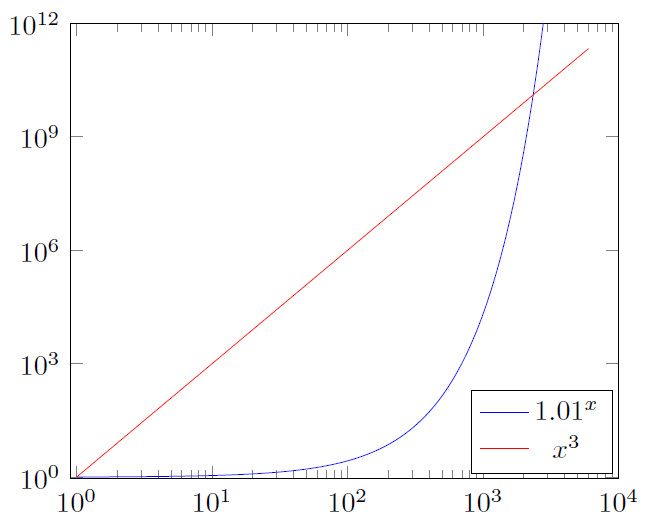
\includegraphics[scale=0.5]{laufzeit/polyVsExp}
\end{frame}

\begin{frame}[t]{Wahr oder Falsch?}
	\TrueQuestionE{$x^4 \in \Oh{{(x^3)}^3}$}{ $ {(x^3)}^3 = x^9$}
	\FalseQuestionE{$\sqrt{n} \in \Om{2^n}$}{}
	\TrueQuestionE{$log_{5000} n \in \Th{\log_2{n^4}}$}{ $ \log_2{n^4} = 4 \cdot \log_2{n}$}
	%
	% ACHTUNG: Sehr aufwendig zu erklären. Besser weglassen, um Zeit zu sparen!
	\FalseQuestionE{$O(f_1) + f_2 = O(f_1 + f_2)$}{Z.~B.: \\ $\Oh{n} + 4 = \set{f(n) + 4 \Mid f(n) \in \Oh{n}} \neq \set{f(n) \Mid f(n) \in \Oh{n}} = \Oh{n+4}$. \\ \textbf{Aber} es gilt: $O(f_1) + O(f_2) = O(f_1 + f_2)$}
\end{frame}

\begin{frame}[t]{Wahr oder Falsch?}
	\FalseQuestion{Für zwei Funktionen $f, g$ gilt immer $f \preceq g$ oder $f \succeq g$.}
	\medskip
	
	\visible<2>{
		Es gibt unvergleichbare Funktionen! Beispiel:
		\begin{align*}
		f(n) &=
		\begin{cases}
		1, & \text{ falls $n$ gerade} \\
		n, & \text{ falls $n$ ungerade} \\
		\end{cases} \\
		g(n) &=
		\begin{cases}
		n, & \text{ falls $n$ gerade} \\
		1, & \text{ falls $n$ ungerade} \\
		\end{cases} \\
		\end{align*}
		Es gilt \textbf{nicht} $g\preceq f$, es gilt \textbf{nicht} $f\preceq
		g$ und es gilt \textbf{erst recht nicht} $f\asymp g$.
	}
\end{frame}
}

\section{Automaten}

\begin{frame}{Endliche Automaten}
	Ein deterministischer endlicher Automat...
	\begin{itemize}
		\item besteht aus endlich vielen Zuständen
		\item ist zu jedem Zeitpunkt in \emph{genau einem} dieser Zustände
		\item wechselt bei Eingabe \emph{genau eines} Zeichens den Zustand in \emph{genau einen, definierten} Folgezustand
		\item und gibt dabei ein Wort als Ausgabe aus
	\end{itemize}

	Die gültigen \enquote{Zustandswechsel} sind als Zustandsübergänge definiert.\\
	\begin{block}{}
		Solche ``DEAs'' kann beispielsweise zum Simulieren von Getränkeautomaten oder auch zur Textsuche und -ersetzung verwenden.
	\end{block}
\end{frame}

\mycomment{ % not enough for its own frame
\begin{frame}{Anwendungen}
	\begin{itemize}
		\item Getränkeautomaten
		\item Textsuche
		\item Textersetzung
	\end{itemize}

	Für Beispiele zur Textsuche und Textersetzung: Übung~12, WS~15/16
\end{frame}
}

\mycomment{ % As a source for copy/pasting:
\begin{tikzpicture}[->,>=stealth,shorten >=1pt,auto,node distance=2.8cm,
semithick,initial text={}]
\tikzstyle{every state}=[fill=red,draw=none,text=white]

\node[initial,state] (A)                    {$q_a$};
\node[state]         (B) [above right of=A] {$q_b$};
\node[state]         (D) [below right of=A] {$q_d$};
\node[state]         (C) [below right of=B] {$q_c$};
\node[state]         (E) [below of=D]       {$q_e$};

\path (A) edge              node {0,1,L} (B)
		  edge              node {1,1,R} (C)
(B) edge [loop above] node {1,1,L} (B)
	edge              node {0,1,L} (C)
(C) edge              node {0,1,L} (D)
	edge [bend left]  node {1,0,R} (E)
(D) edge [loop below] node {1,1,R} (D)
	edge              node {0,1,R} (A)
(E) edge [bend left]  node {1,0,R} (A);
\end{tikzpicture}	
}

%\subsection{Mealy-Automaten}
\mycomment{ % see frame below for introduction with moore
\begin{frame}{Ein einfacher Automat}
	\begin{center}
		\begin{tikzpicture}[->,>=stealth,shorten >=1pt,auto,node distance=2.8cm,
			semithick,initial text={}]
			\tikzstyle{every state}=[]
			
			\node[initial,state] (A)                    {$a$};
			\node[state]         (M) [right of=A] 	    {$m$};
			
			\path (A) edge [loop above] node {$\word 1\io\word 0$} (A)
			          edge [loop below]  node {$\word 0\io\word 1$} (A)
			          edge 					  node {$\word{2}\io\word{X}$} (M)
			      (M) edge [loop right] node {$\stackedtight{\word 0\io\word X \\ \word 1\io\word X \\ \word 2\io\word X}$} (M);
			      %(M) edge [loop right] node {\word 1|\word X} (M)
			      %(M) edge [loop below] node {\word 2|\word X} (M);
		\end{tikzpicture}
	\end{center}
	\pause
	Eingabe: \word{011101} \?> Ausgabe: \word{100010} \\
	Eingabe: \word{011102} \?> Ausgabe: \word{10001X} \\
	Eingabe: \word{012101} \?> Ausgabe: \word{10XXXX} \\ \pause
	\smallskip
	\impl Der Automat negiert das Eingabewort bitweise. \\
	(Frisst er ne \word 2, so isser beleidigt. \smiley)
\end{frame}
}

\subsection{Moore-Automaten}
\begin{frame}{Ein einfacher Automat}
	\begin{center}
		\begin{tikzpicture}[->,>=stealth,shorten >=1pt,auto,node distance=2.8cm,
			semithick,initial text={}]
			\tikzstyle{every state}=[]
			
			\node[initial,state] (A)                    {$a\io$ \smiley};
			\node[state]         (M) [right of=A] 	    {$m\io$ \frownie};
			
			\path (A) edge [loop above] node {$\word 1$} (A)
			          edge [loop below]  node {$\word 0$} (A)
			          edge 					  node {$\word{2}$} (M)
			      (M) edge [loop right] node {$\word{0}, \word{1}, \word{2}$} (M);
			      %(M) edge [loop right] node {\word 1|\word X} (M)
			      %(M) edge [loop below] node {\word 2|\word X} (M);
		\end{tikzpicture}
	\end{center}
	\pause
	Eingabe: \word{011101} \?> Ausgabe: \word{\smiley\smiley\smiley\smiley\smiley\smiley} \\
	Eingabe: \word{011102} \?> Ausgabe: \word{\smiley\smiley\smiley\smiley\smiley\frownie} \\
	Eingabe: \word{012101} \?> Ausgabe: \word{\smiley\smiley\frownie\frownie\frownie\frownie} \\ \pause
	\smallskip
	\impl Der Automat prüft, ob die Eingabe nur aus binären Ziffern besteht. \\
	(Frisst er ne \word 2, so isser beleidigt. \frownie)
\end{frame}

\mycomment{ % i can't do this any moore
\begin{frame}{Mealy-Automat}
	Bei einem Mealy-Automaten findet die Ausgabe \textbf{bei den Zustandsübergängen} statt.
	\begin{Definition}
		Ein \textbf{Mealy-Automat} $ A = (Z,z_0,X,f,Y,g)$ besteht aus...
		\begin{itemize}
			\item einer endlichen Zustandsmenge $Z$ 
			\item einem Startzustand $z_0$
			\item einem Eingabealphabet $X$ 
			\item einer Zustandsübergangsfunktion $f \from Z\times X \functionto Z $
			\item einem Ausgabealphabet $Y$
			\item einer Ausgabefunktion $g \from Z\times X \functionto Y^* $ 
		\end{itemize}						
	\end{Definition}
\end{frame}
}

\begin{frame}{Moore-Automat}
	Bei einem Moore-Automaten findet die Ausgabe \textbf{in den Zuständen} statt.
	\begin{Definition}
		Ein \textbf{Moore-Automat} $ A = (Z,z_0,X,f,Y,g)$ besteht aus...
		\begin{itemize}
			\item einer endlichen Zustandsmenge $Z$ 
			\item einem Startzustand $z_0 \in Z$
			\item einem Eingabealphabet $X$ 
			\item einer Zustandsübergangsfunktion $f \from Z\times X \functionto Z $
			\item einem Ausgabealphabet $Y$
			\item einer Ausgabefunktion $h \from Z \functionto Y^* $ 
		\end{itemize}						
	\end{Definition}
\end{frame}

\mycomment{ % another one
\begin{frame}{}
	\begin{block}{Graphische Darstellung}
		\begin{itemize}
			\item Oft malt man Automaten hin. (Achtung: Die formale Schreibweise wird trotzdem auch im Studium verwendet! Also auswendig lernen!)
			\item Zustände sind \textbf{Knoten} und Übergänge sind \textbf{gerichtete Kanten} in einem Graphen. \\
			Kanten\textbf{beschriftung}: „$\langle\text{Eingabe}\rangle | \langle\text{Ausgabe}\rangle$“
			\item \textbf{Der Startzustand wird mit einem Pfeil \enquote{aus dem Nichts} gekennzeichnet!}  \pause
			\implitem \textbf{NICHT VERGESSEN!} Kostet sonst Punkte! \textbf{Immer!}
		\end{itemize}
		
	\end{block}
\end{frame}
}

\begin{frame}{Moore-Automat}
	\begin{block}{Graphische Darstellung}
		\begin{itemize}
			\item Oft malt man Automaten hin. (Achtung: Die formale Schreibweise wird trotzdem auch im Studium verwendet! Also auswendig lernen!)
			\item Zustände sind \textbf{Knoten} und Übergänge sind \textbf{gerichtete Kanten} in einem Graphen.
			\item[] Knotenbeschriftung: „$\langle\text{Zustand}\rangle | \langle\text{Ausgabe}\rangle$“
			\item[] Kantenbeschriftung: „Eingabe“ des Übergangs
			\item \textbf{Der Startzustand wird mit einem Pfeil \enquote{aus dem Nichts} gekennzeichnet!}  \pause
			\implitem \textbf{NICHT VERGESSEN!} Kostet sonst Punkte! \textbf{Immer!}
		\end{itemize}
		
	\end{block}
\end{frame}

\mycomment{ % mealy no
\begin{frame}{Beispiel: Automatengraphen}
	%\vspace{-1\baselineskip} 
	%\hspace{-\baselineskip}
	
\includegraphics[page=3,trim=18px 47px 18px 14px,clip]{U12.pdf}	
\end{frame}
}

% moore yes
\begin{frame}{Beispiel Moore-Automat}
	
\includegraphics[page=11,trim=18px 47px 18px 13px,clip]{U12.pdf}	
\end{frame}

%% Übung: Beispiel
%\setbeamercolor{background canvas}{bg=}


\begin{frame}{Eingabe eines Zeichens}
	Was ist die Zustandsübergangsfunktion $f$? \\ \pause
	\medskip
	Haben
	\begin{itemize}
		\item aktuellen Zustand $z \in Z$
		\item eingelesenes Zeichen $x \in X$
	\end{itemize}
	\impl $f$ liefert den Folgezustand $z_\text{neu}$, in welchem der Automat danach ist.\\
	\medskip
	Formell: $$ f(z,x) = z_\text{neu} $$ 
\end{frame}

\begin{frame}{Eingabe eines Wortes}
	Was machen wir mit ganzen Wörtern? \\ \pause
	Wir definieren uns ganz analog
	\begin{block}{Zustandsübergangsfunktion extended}
	\begin{align*}
		 	f_*(z,\eps) &:= z \\
		 	\forall w\in X^* , \, x\in X : \quad  f_*(z,wx) &:= f\left(f_*(z,w),x\right) 
	\end{align*}
	\end{block}
	\pause Was macht diese Funktion? \\ \pause
	\medskip
	Haben
	\begin{itemize}
		\item aktuellen Zustand $z \in Z$
		\item eingelesenes Wort $w \in X^*$
	\end{itemize}
	\impl $f_*$ liefert den \textbf{Endzustand} $z_\text{ende}$, in welchem der Automat \textbf{nach dem Wort} dann ist.
	Formell: $$ f_*(z,w) = z_\text{ende} $$
	%Bei Eingabe eines Wortes $w$ und Anfangszustand $z$ gibt sie den Zustand $z' = f_*(z,w)$ aus, in dem der Automat enden wird. 
\end{frame}
	
\begin{frame}{Eingabe eines Wortes}
	Definieren wir nun weiter 
	\begin{block}{Zustandsübergangsfunktion extended extended}
		\begin{align*}
			f_{**}(z, \eps) &:= z \\
			\forall w\in X^* , \, x\in X : \quad  f_{**}(z, xw)   &:= z \cdot f_{**}\!\left(f(z,x),w\right) \\
		\end{align*}
	\end{block}
	\pause Was macht diese Funktion? \\ \pause
	Diese Funktion gibt die Reihe aller \textbf{Zustände als Gesamtwort} aus, die der Automat bei Eingabe des Wortes $w$ im Startzustand $z$ durchläuft. Also: 
	$$ f_{**}(z, w) = z \* z_1 \* z_2 \cdots z_\text{ende} $$
\end{frame}

\begin{frame}{Eingabe eines Wortes}		
	Alternative Definition:
	\begin{block}{Zustandsübergangsfunktion extended extended}
		\begin{align*}
			f_{**}(z,\varepsilon) &= z \\
			\forall w \in X^* \ \forall x \in X : f_{**}(z,wx) &= f_{**}(z,w)\cdot f(f_*(z,w),x)	 
		\end{align*}
	\end{block}
\end{frame}

\begin{frame}{Beispiel $f, f_*, f_{**}$}
	\begin{center}
		\begin{tikzpicture}[->,>=stealth,shorten >=1pt,auto,node distance=2.8cm,
			semithick,initial text={}]
			\tikzstyle{every state}=[]
			
			\node[initial,state] (A)                    {$a\io$ \smiley};
			\node[state]         (M) [right of=A] 	    {$m\io$ \frownie};
			
			\path (A) edge [loop above] node {$\word 1$} (A)
			          edge [loop below]  node {$\word 0$} (A)
			          edge 					  node {$\word{2}$} (M)
			      (M) edge [loop right] node {$\word{0}, \word{1}, \word{2}$} (M);
			      %(M) edge [loop right] node {\word 1|\word X} (M)
			      %(M) edge [loop below] node {\word 2|\word X} (M);
		\end{tikzpicture}
	\end{center}
	\begin{align*}
		f(a, \word 2) &= m \\
		f(a, \word 0) &= a \\ 
	\end{align*}
	\pause  \vspace{-2.5\baselineskip}
	\begin{align*}
		f_*(a, \word{101}) &= \hphantom{aaa}a \\
		f_{**}(a, \word{101}) &= aaaa \\ 
	\end{align*}
	\pause  \vspace{-2.5\baselineskip}
	\begin{align*}
		f_*(a, \word{1021}) &= \hphantom{aaam}m \\
		f_{**}(a, \word{1021}) &= aaamm
	\end{align*}
\end{frame}

\mycomment{ % we dont do that here
\begin{frame}{Ausgaben}
	Automaten können ja was ausgeben. \\
	\smallskip
	Erinnerung: Die Kanten sind beschriftet mit $x \io y$ , wobei $x\in X$ und $y\in Y^* $. \\
	 \impl Für Eingabe $x$ wird das Wort $y$ ausgegeben. \\ 
	Formal: $$g(z,x) = y$$
\end{frame}

\begin{frame}{Ausgabefunktionen}
	\begin{block}{Ausgabefunktion extended}
		Wir können also analog zu $f_*$ und $f_{**}$ definieren
		\begin{threealign}
		\text{Für die letze Ausgabe: } \qquad g_* : Z\times X^* &\functionto& Y^* \\
		g_*(z,\varepsilon) &=& \varepsilon \\
		\forall w\in X^* \; \forall x\in X : g_*(z,wx) &=& g(f_*(z,w),x) \\ \\
		\text{Für das ganze Ausgabewort: } \qquad g_{**} : Z\times X^* &\functionto& Y^* \\ 
		g_{**}(z,\varepsilon) &=& \varepsilon \\
		\forall w\in X^* \; \forall x\in X : g_{**}(z,wx) &=& g_{**}(z,w)\cdot g_*(z,wx) 			
		\end{threealign} 
	\end{block}
	
	%\pause Dies gibt nun nicht die durchlaufenen Zustände bzw. den Abschlusszustand an, sondern die letzte Ausgabe bzw. alle durchlaufenen Ausgaben. 

\end{frame}
}

\begin{frame}{Ausgaben}
	Automaten können ja was ausgeben. \\
	\smallskip
	Erinnerung: Die Knoten sind beschriftet mit $z \io y$ , wobei $z\in Z$ und $y\in Y^* $. \\
	 \impl Beim Betreten von Zustand $z$ wird das Wort $y$ ausgegeben. \\ 
	Formal: $$h(z) = y$$
\end{frame}

\begin{frame}{Ausgabefunktionen}
	\begin{block}{Ausgabefunktion extended}
		Wir können also analog zu $f_*$ und $f_{**}$ definieren
		\begin{threealign}
		\text{Für die letze Ausgabe: } \qquad g_* : Z\times X^* &\functionto& Y^* \\
		g_*(z,w) &=& h(f_*(z,w)) \\
		\text{Für das ganze Ausgabewort: } \qquad g_{**} : Z\times X^* &\functionto& Y^* \\ 
		g_{**}(z,w) &=& h^{**}(f_{**}(z,w)) \\
		\end{threealign} 
		Dabei ist $h^{**}\from Z^*\functionto Y^*$ der durch $h$ induzierte Homomorphismus!
	\end{block}
	
	%\pause Dies gibt nun nicht die durchlaufenen Zustände bzw. den Abschlusszustand an, sondern die letzte Ausgabe bzw. alle durchlaufenen Ausgaben. 

\end{frame}

\begin{frame}{Beispiel $g, g_*, g_{**}$}
	\begin{center}
		\begin{tikzpicture}[->,>=stealth,shorten >=1pt,auto,node distance=2.8cm,
			semithick,initial text={}]
			\tikzstyle{every state}=[]
			
			\node[initial,state] (A)                    {$a\io$ \smiley};
			\node[state]         (M) [right of=A] 	    {$m\io$ \frownie};
			
			\path (A) edge [loop above] node {$\word 1$} (A)
			          edge [loop below]  node {$\word 0$} (A)
			          edge 					  node {$\word{2}$} (M)
			      (M) edge [loop right] node {$\word{0}, \word{1}, \word{2}$} (M);
			      %(M) edge [loop right] node {\word 1|\word X} (M)
			      %(M) edge [loop below] node {\word 2|\word X} (M);
		\end{tikzpicture}
	\end{center}
	\vspace{-\baselineskip}
	\begin{align*}
	g(a, \word 2) &= \word \frownie \\
	g(a, \word 0) &= \word \smiley \\ 
	\end{align*}
	\pause  \vspace{-2.5\baselineskip}
	\begin{align*}
	g_*(a, \word{101}) &= \hphantom{\word{\smiley\smiley}}\word \smiley \\
	g_{**}(a, \word{101}) &= \word{\smiley\smiley\smiley} \\ 
	\end{align*}
	\pause  \vspace{-2.5\baselineskip}
	\begin{align*}
	g_*(a, \word{1021}) &= \hphantom{\word{\smiley\smiley\frownie}}\word \frownie \\
	g_{**}(a, \word{1021}) &= \word{\smiley\smiley\frownie\frownie} \\ 	\visible<+->{}
	\visible<+->{g_*(m, \word{0110}) &= }\visible<+->{\word \frownie}
	\end{align*}
\end{frame}


\mycomment{ % no need to declare differences if we only have one
\subsection{Moore-Automat}
\begin{frame}{Moore-Automat}
	Moore-Automaten sind fast genauso aufgebaut wie Mealy-Automaten.\\ \smallskip
	\textbf{Unterschied}: Ausgabe erfolgt „\textbf{im Zustand}“, nicht beim Zustandsübergang. \\ \pause 
	\begin{tabular}{cc}
		Mealy: & Moore: \\
		\begin{tikzpicture}[->,>=stealth,shorten >=1pt,auto,node distance=2.8cm,
		semithick,initial text={}]
		\tikzstyle{every state}=[]
		
		\node[state,white] (X)                    {\hphantom{XXX}};
		\node[state]         (A) [right of=X] 	    {$A$};
		
		\path (X) edge [bend left=9]	 node {$\word a\io\word 0$} (A)
				  edge [bend right=9]	 node [below] {$\word b\io\word 1$} (A);
		\end{tikzpicture}
		&
		\begin{tikzpicture}[->,>=stealth,shorten >=1pt,auto,node distance=2.8cm,
		semithick,initial text={}]
		\tikzstyle{every state}=[]
		
		\node[state,white] (X)                    {\hphantom{XXX}};
		\node[state]         (A) [right of=X] 	    {$A\io\word{XY}$};
		
		\path (X) edge [bend left=9]	 node {\word a } (A)
				  edge [bend right=9]	 node [below] {\word b } (A);
		\end{tikzpicture}
	\end{tabular} \\
	\pause
	Ausgabefunktion heißt jetzt also auch: $$h\from Z\functionto Y^*$$ \impl Ausgabe hängt \textbf{nicht} von der Eingabe ab!\\
\end{frame}

\begin{frame}{Moore-Automat – Ausgabe}
	Ausgabefunktion heißt jetzt also auch: $$h\from Z\functionto Y^*$$ \impl Ausgabe hängt \textbf{nicht} von der Eingabe ab!\\ 
	Dann def. wir $$ g_* (z,w) := h(f_*(z,w)) $$
	\pause
	Für $g_{**}$ gilt dann mit $h^{**}\from Z^*\functionto Y^*$ \quad (der durch $h$ induzierte Hom.!)  $$ g_{**}(z,w) = h^{**} (f_{**}(z,w)) $$
	Wir wenden also $h$ auf jeden durchlaufenen Zustand an.
\end{frame}
}


\mycomment{ % we already did this
\begin{frame}{Beispiel Moore-Automat}
	
\includegraphics[page=11,trim=18px 47px 18px 13px,clip]{U12.pdf}	
\end{frame}
}

\mycomment{% no mealy in WT20/21
\begin{frame}{Umwandlung von Automaten: Moore $\leftrightsquigarrow$ Mealy}
	\begin{block}{Von Moore zu Mealy}
		Relativ straightforward.\\
		Ausgaben \enquote{aus den Knoten auf die Übergänge ziehen}\\
		\medskip
		\textbf{Beachte}: Für die Eingabe $\eps$ kann ein Moore-Automat eine Ausgabe $g_{**}(s, \eps) \neq \eps$ erzeugen, ein Mealy-Automat \emph{jedoch nicht}.
	\end{block}

	\begin{block}{Von Mealy zu Moore}
		Komplizierter.
	\end{block}
\end{frame}

\begin{frame}{Beispiel: Umwandlung von Mealy nach Moore}
	%\vspace{-2\baselineskip}
	\begin{tikzpicture}[->,>=stealth,shorten >=1pt,auto,node distance=2.8cm,
	semithick,initial text={}]
	\tikzstyle{every state}=[]
	
	\node[initial,state] (A)                    {$a$};
	\node[state]         (M) [right of=A] 	    {$m$};
	
	\path (A) edge [loop above] node {$\word 1\io\word 0$} (A)
	edge [loop below]  node {$\word 0\io\word 1$} (A)
	edge 					  node {$\word{2}\io\word{X}$} (M)
	(M) edge [loop right] node {$\stackedtight{\word 0\io\word X \\ \word 1\io\word X \\ \word 2\io\word X}$} (M);
	\end{tikzpicture}
	\\
	\pause  
	\vspace{-1\baselineskip}
	%\mbox{}\hspace{.6\textwidth} 
	\begin{tikzpicture}[->,>=stealth,shorten >=1pt,auto,node distance=2.1cm,
	semithick,initial text={}]
	\tikzstyle{every state}=[]
	
	\node[initial,state] (A)                    {$a\io\eps$};
	\node[state]         (B) [above right of=A] 	    {$b\io\word 0$};
	\node[state]         (C) [below right of=A] 	    {$c\io\word 1$};
	\node[state]         (M) [below right of=B] 	    {$m\io\word X$};
	
	\path 
		(A) edge 				node {\word 1} (B)
		(A) edge 				node [below] {\word 0} (C)
		(B) edge [bend left=8]	node {\word 0} (C)
		(B) edge [loop right]   node {\word 1} (B)
		(C) edge [bend left=8]	node {\word 1} (B)
		(C) edge [loop right]   node {\word 0} (C)
		(B) edge 				node {\word 2} (M)
		(C) edge 				node [below] {\word 2} (M)
		(M) edge [loop right]	node {\word 0, \word 1, \word 2} (M)
	;
	\draw[->] (A) to[out=-90,in=-76, looseness=1.94] (M) node [at start, below right = 48pt and 2pt] {\word 2}; %Fuck you, LaTeX. "midway" node option doesn't work at all. Beware: `below=48pt, right=2pt` doesn't seem to work anymore?! WTF!?
	\end{tikzpicture}
\end{frame}
} % end mycomment

\mycomment{ % for tut 13
\begin{frame}{Aufgabe: Zeichen duplizieren}
	\begin{block}{Aufgabe}
		Malt einen Moore-Automaten, der für eine Eingabe $w \in \{\word{a},\word{b},\word{c}\}$ jedes Eingabezeichen ``verdoppelt'', also z.B. $\word{abac}$ wird zu $\word{aabbaacc}$ \\
		\pause
		\bigskip
	\end{block}
	%\vspace{-2\baselineskip}
	\begin{tikzpicture}[->,>=stealth,shorten >=1pt,auto,node distance=2.8cm,
	semithick,initial text={}]
	\tikzstyle{every state}=[]
	
	\node[initial,state] (1)                    {$1\io\word{aa}$};
	\node[state]         (2) [right of=1] 	    {$2\io\word{bb}$};
	\node[state]         (3) [right of=2] 	    {$3\io\word{cc}$};
	
	\path (1) edge [loop above] node {$\word a$} (1)
			edge [bend left=12] node {$\word b$} (2)
			edge [bend right=30] node {$\word c$} (3)
		(2) edge [loop above] node {$\word b$} (2)
			edge [bend left=12] node {$\word a$} (1)
			edge [bend left=12] node {$\word c$} (3)
		(3) edge [loop above] node {$\word c$} (3)
			edge [bend left=36] node {$\word a$} (1)
			edge [bend left=12] node {$\word b$} (2);
	\end{tikzpicture}
\end{frame}

\begin{frame}{Aufgabe: Textersetzung mit Automaten}
	\begin{block}{Aufgabe}
		Geg.: \quad $w \in \set{\word a, \word b}^*$, wobei $w$ nicht auf ungerade viele \word{a} endet. \\
		Wollen \word{aa} durch \word{ccc} ersetzen. \\
		Malt einen Moore-Automaten, der das leistet. \\
		\pause
		\bigskip
	\end{block}
	%\vspace{-2\baselineskip}
	\begin{tikzpicture}[->,>=stealth,shorten >=1pt,auto,node distance=2.8cm,
	semithick,initial text={}]
	\tikzstyle{every state}=[]
	
	\node[initial,state] (1)                    {$1$};
	\node[state]         (2) [right of=A] 	    {$2$};
	
	\path (1) edge [loop above] node {$\word b\io\word b$} (1)
	% edge [loop below]  node {$\word 0\io\word 1$} (A)
	edge 	[bend left=12]				  node {$\word{a}\io\eps$} (2)
	(2) edge [bend left=12] node  {$\stackedtight{\word b\io\word{ab} \\ \word a\io\word{ccc}}$} (1);
	\end{tikzpicture} \\
	Zustand 2 „merkt sich“, dass ein einzelnes \word a gelesen wurde. \\
	\pause
	\medskip
	\Impl Beispiel:  $g_{**}(1, \word{babaabaa}) = \word{babcccbccc}$.
	% Einschränkungen von oben mit ba und so nötig, weil sonst das letzte a nicht ausgegeben wird (möglicher Fix: Ein End-of-Input-Zeichen, das am Ende „aufräumt“)
\end{frame}
}

\mycomment{
\only<beamer:0>{

\begin{headframe}[\daniel{Zu hässlich zum Wegwerfen}]
	Unübersichtliche Beispiele
\end{headframe}

\begin{frame}{Beispiel: Ein Getränkeautomat}
	$\word R$ sei reines Wasser, $\word Z$ ist Zitronenlimonade, $\word O$ ist OK (Getränkeausgabe), $\word C$ ist Clear und $\word 1$ entspricht einer 1-€-Münze. (\word - heißt „kein Getränk ausgewählt“)\\
	Wir wollen: \pause
	\begin{itemize}[<+->]
		\item Getränk wählen können
		\item Geld rein- und rausholen können
		\item und immer zurück kommen können! ($=$ Abbruch-Knopf)
	\end{itemize}
\end{frame}

\begin{frame}
	\begin{figure}[H]
		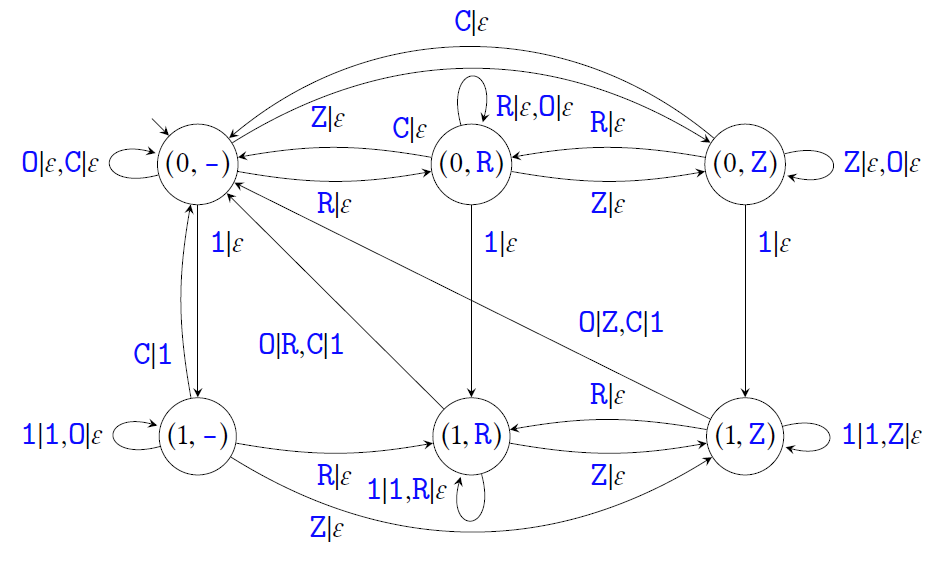
\includegraphics[scale=0.4]{automaten/getraenke} % ist „ohne Ausgabe“ überhaupt erlaubt?? Ich denke nicht.
	\end{figure}
	
	Was ist $f((0,\word -), \word Z), \, f_*((0,\word -), \word{R10}) ,  \, f_{**}( (0,\word -),\word{R10}) $ ? Rechnerisch und graphisch.	
	
\end{frame}

\begin{frame}
	Rechnerisch nur der 3. Fall:
	\begin{threealign}
	f_{**}((0,\word -),\word{R10}) &=& f_{**}((0,\word -),\word{R1}) )\cdot f(f_*((0,\word -),\word{R1}),\word{0}) \\ 
	&=& f_{**} ((0,\word -),\word R) \cdot f(f_*((0,\word -),\word R),\word 1) \\& & \mbox{} \cdot f(f_*((0,\word -),\word{R1}),\word 0) \\ 
	&=& f_{**}((0,\word -),\eps) \cdot f(f_*((0,\word -),\eps),\word R) \\ &&\mbox{} \cdot f(f_*((0,\word -),\word R),\word 1) \cdot f(f_*((0,\word -),\word{R1}),\word 0) \\ 
	&=& (0,\word -) \cdot f((0,\word -),\word R) \cdot f( f(f_*((0,\word -),\eps),\word R),\word 1) \\ &&\mbox{} \cdot f( f(f_*((0,\word -),\word R),\word 1),\word 0) \\
	&=& (0,\word -) \cdot f((0,\word -),\word R) \cdot f( f((0,\word -),\word R),\word 1)  \\& &\mbox{} \cdot f(f(  f(f_*(0,\word -),\eps),\word R),\word 1), \word 0) \\
	&=& (0,\word -) \cdot f((0,\word -),\word R) \cdot f( f((0,\word -),\word R),\word 1)\\ &&\mbox{} \cdot f( f(f((0,\word -),\word R),\word 1),\word 0) \\ 
	&=& (0,\word -) \cdot (0,\word R) \cdot (1,\word R) \cdot (0,\word -) 
	\end{threealign} 
\end{frame}

\begin{frame}{Beispiel}
	\begin{figure}[H]
		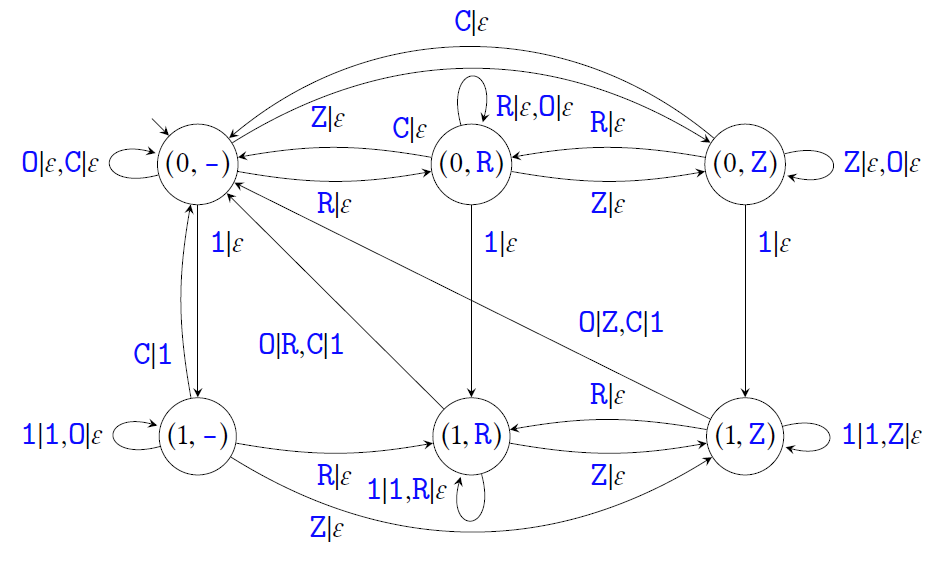
\includegraphics[scale=0.4]{automaten/getraenke}			
	\end{figure}
	Was ist $g_*((0,\word -), \word{R10}) , \, g_{**}((0,\word -),\word{R10}) , \, g_{**}((0,\word -),\word{R110}) $ ? \\ \pause
	$g_*((0,\word -),\word{R10}) = g_{**}((0,\word -),\word{R10}) = \word R, \qquad g_{**}((0,\word -),\word{R110}) = \word{1R} $	
\end{frame}

\begin{frame}{}
	Beispiel: Automaten-Umwandlung (Übung 12, WS 15/16)
\end{frame}

%% Übung: Beispiel
\setbeamercolor{background canvas}{bg=}

\includepdf[pages={34-40}]{U12.pdf}
}
} % end mycomment

\section{Endliche Akzeptoren}
\begin{frame}[t]{Endliche Akzeptoren}
	\begin{Definition}
		Ein \textbf{endlicher Akzeptor} $A$ ist ein \emph{Moore}-Automat mit Ausgabealphabet $ Y= \{\word 0,\word 1\}$, der zuletzt $\word 1$ ausgibt, falls ihm das Wort gefällt und \word 0 sonst.
	\end{Definition} 
	
	$A$ \textbf{akzeptiert} ein Wort $w$, wenn er als Letztes eine $\word 1$ ausgibt. \\ \medskip 
	
	\only<all:2>{
		\begin{center}
					\begin{tikzpicture}[->,>=stealth,shorten >=1pt,auto,node distance=1.8cm,
				semithick,initial text={}]
				\tikzstyle{every state}=[]
				
				\node[state] (A)                    {$a\io\word 0$};
				\node[state] (B) [right of=A] 	    {$b\io\word 1$};
				
				\end{tikzpicture}
		\end{center}
	}
	\only<all:3>{
		\begin{center}
					\begin{tikzpicture}[->,>=stealth,shorten >=1pt,auto,node distance=1.8cm,
				semithick,initial text={}]
				\tikzstyle{every state}=[]
				
				\node[state] (A)                    {$a$};
				\node[state, accepting] (B) [right of=A] {$b$};
				
				\end{tikzpicture}
		\end{center} 
		\emph{Notation:} Wir nennen die Menge der \textbf{akzeptierenden Zustände} $F$ und malen solche mit einem Doppelkreis. \\ 
	}
\end{frame}

\begin{frame}{Von einem Akzeptor erkannte Sprache}
	Wir sprechen von einer \textbf{akzeptierten Sprache} über einem Alphabet. Sie ist definiert als 
	\begin{align*}
		L(A) &:= \{ w \mid f_*(z_0,w) \in F \}  \\
			 &\: = \{ w \mid g_*(z_0,w) = \word 1 \}.
	\end{align*}
	Also sind in einer akzeptierten Sprache alle Wörter, die von $A$ akzeptiert werden. \pause
	
	\begin{Beispiel}
		Sei $A$ gegeben als
		\vspace{-2\baselineskip}
		\begin{center}
			\begin{tikzpicture}[->,>=stealth,shorten >=1pt,auto,node distance=1.8cm,
			semithick,initial text={}]
			\tikzstyle{every state}=[]
			
			\node[initial, state, accepting] (A)                    {$z_0$};
			\node[state] (B) [right of=A] {$z_1$};
			
			\path
				(A) edge [loop above] node {\word a, \word b}  (A)
					edge [bend right=7] node [below] {\word c} 		  (B)
				(B) edge [loop right] node {\word c}		  (B)
					edge [bend right=7] node [above] {\word a, \word b} (A)
			;
			\end{tikzpicture}. % Sätze enden mit nem Punkt! :D
		\end{center} 
		\pause
		Dann ist $L(A) = \set{w \in \set{\word a, \word b, \word c}^* \Mid \text{$w$ endet nicht auf \word c}}$.
	\end{Beispiel}
\end{frame}

\begin{frame}{Aufgaben}
	Gebt einen Akzeptor an, der die Sprache aller Binärzahlen erkennt, die Zweierpotenzen darstellen. 
	\pause ($= \set{\word 0}^* \* \set{\word 1} \* \set{\word 0}^*$) \\
	%\vspace{-2\baselineskip}
	\begin{center}
		\begin{tikzpicture}[->,>=stealth,shorten >=1pt,auto,node distance=2cm,
		semithick,initial text={}]
		\tikzstyle{every state}=[]
		
		\node[initial,state] (A)                    {$a$};
		\node[state,accepting] (B)  [right of=A]     {$b$};
		\node[state]		 (M)  [right of=B]		{$m$};
		
		\path
		(A) edge [loop above]  node {\word 0} (A) 
		(A) edge 			  node {\word 1} (B) 
		(B) edge [loop above]  node {\word 0} (B) 
		(B) edge 			  node {\word 1} (M) 
		(M) edge [loop above] node {\word 0, \word 1} (M);
		\end{tikzpicture}
	\end{center}
	\pause
	\begin{block}{Bonusaufgabe}
		Gebt einen Akzeptor an, der die Sprache aller geraden Binärzahlen erkennt. 
		\pause ($= \set{\word 0,\word 1}^* \* \set{\word 0}$) \\
		%\vspace{-2\baselineskip}
		\begin{center}
			\begin{tikzpicture}[->,>=stealth,shorten >=1pt,auto,node distance=1.8cm,
			semithick,initial text={}]
			\tikzstyle{every state}=[]
			
			\node[initial, state] (A)                    {$a$};
			\node[state, accepting] (B) [right of=A] {$b$};
			
			\path
			(B) edge [loop above] node  {\word 0}  (B)
				edge [bend right=7] node [above] {\word 1} 		  (A)
			(A) edge [loop above] node  {\word 1}		  (A)
				edge [bend right=7] node [below] {\word 0} (B)
			;
			\end{tikzpicture}
		\end{center} 
	\end{block}
\end{frame}

\begin{frame}{Aufgabe}
	Der endliche Akzeptor $A = (Z, z_0, X, f, F)$ sei gegeben durch
	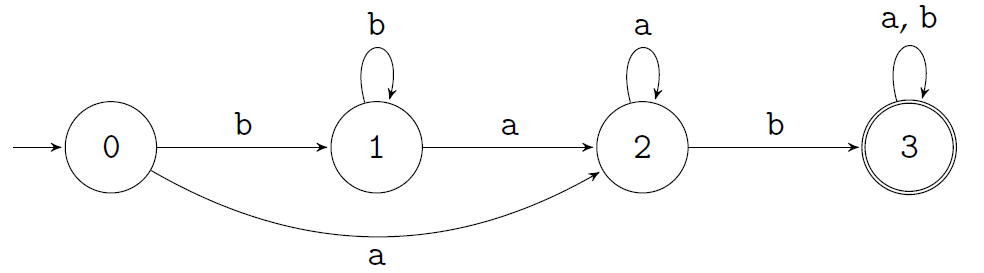
\includegraphics[scale=0.4]{automaten/akz1516B12A1}
	
	Gebt die von $A$ akzeptierte Sprache $L(A)$ unter ausschließlicher Benutzung der formalen Sprachen $\{\word a\}$, $\{\word b\}$, sowie $\{\word a, \word b\}$, des Konkatenationsabschlusses und des Produkts formaler Sprachen an.
	
	\emph{Beispiel:} $\{\word a, \word b\}^* \cdot \{\word a\} \cdot \{\word b\}$
	
	\visible<2-|handout:2>{
		\begin{block}{Lösung}
			$L(A) = \{\word b\}^* \cdot \{\word a\} \cdot \{\word a\}^* \cdot \{\word b\} \cdot \{\word a, \word b\}^*$ \\
			$\hphantom{L(A) } = \{\word b\}^* \cdot \hphantom{\{\word a\} \cdot \mbox{}} \{\word a\}^+ \!\cdot \{\word b\} \cdot \{\word a, \word b\}^*$
		\end{block}
	}
\end{frame}

\begin{frame}{Bonusaufgabe}
	\begin{enumerate}[a)]
		\item Zeichnet einen möglichst kleinen endlichen Akzeptor mit $ X = \{\word a, \word b\}$, der alle Wörter akzeptiert, bei denen die Anzahl der $\word a$ durch $5$ teilbar ist.
		\item Zeichnet einen Akzeptor mit $ X = \{\word a,\word b\}$, der alle Wörter akzeptiert, in denen nirgends hintereinander zwei $\word b$ vorkommen.
	\end{enumerate}		
\end{frame}

\begin{frame} {Lösung Bonusaufgabe a)}
	\begin{figure}[H] 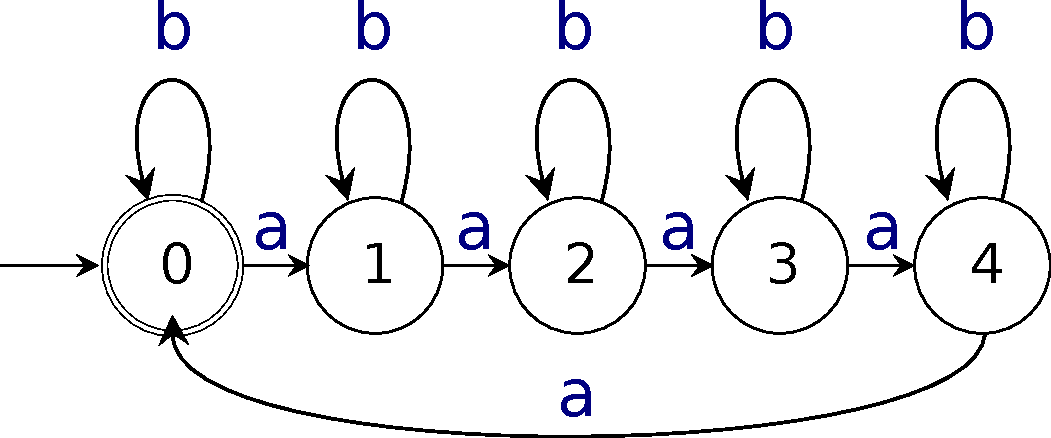
\includegraphics[scale=0.5]{automaten/Akzeptor1.pdf} \end{figure}		
\end{frame} 

\begin{frame}{Lösung Bonusaufgabe b)}
	\begin{figure}[H] 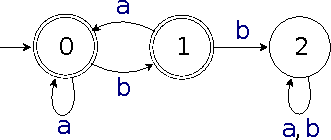
\includegraphics[scale=1.5]{automaten/Akzeptor2.pdf} \end{figure}
\end{frame}



% No longer todo: Fix dirty hack in thwregex.sty, where I changed line 42 to print star in math-mode
% 		because otherwise the star was always raised in my config.
%	COmment(Daniel): Reverted your change. No problems whatsoever.
%		Use \rx everywhere

% Fuck you, Latex. In my algo tutorial slides, this isn't necessary. Why here then!?
\begin{frame}[t]
	\fakeframetitle{\only<2->{Grenzen endlicher Akzeptoren}}
	Gibt es einen endlichen Akzeptor $A$ mit $$L(A) = \set{ \word a^k\word b^k \Mid k\in \N_0 }?$$
	\pause
	Nein! Warum nicht? \visible<3->{Endliche Automaten können nicht unendlich weit „zählen“!}\\
	
	Gibt es einen endlichen Akzeptor, der alle gültigen Klammerausdrücke erkennt?\\ \pause
	Nein, aus dem selben Grund.
	\begin{figure}[H]
		\centering
		
\includegraphics[scale=0.5]{xkcd/tags_1144}
		{ {\url{https://www.xkcd.com/1144/}} }
	\end{figure}
	\pause
	Kontextfreie Grammatiken \enquote{können also mehr} als endliche Akzeptoren.\\
	Wir wollen nun ein \enquote{gleichmächtiges} Konzept zu Akzeptoren.
\end{frame}

\section{Reguläre Ausdrücke}
\subsection{Definition}

\begin{frame}{Disclaimer!}
	\begin{center}
		\Large
			\bfalert{\Huge ACHTUNG!} \\ \medskip
		
		Gemeint sind \textbf{NICHT} sog. \emph{Regular Expressions}, die ihr vllt. aus Programmiersprachen kennt! \\ \bigskip
		
		{\normalsize (Die sind ähnlich, aber eben nicht das gleiche.)}
	\end{center}
\end{frame}

\begin{frame}{Reguläre Ausdrücke} 
	Bislang: Beschreibung der Sprache $L$ eines endlichen Akzeptors aus einzelnen Mengen, Vereinigung, Konkatenation, \dots \\
	$$ L = (\set{\word{ab}} \cdot \set{\word c, \word d})^\ast \cup \set{\word e}$$
	\medskip \pause
	
	Jetzt: Ein Ausdruck $R$, um eine mit solchen Operationen \enquote{zusammengebaute} Sprache zu beschreiben.\\
	$$ R = \rx{(ab(c|d))*|e}$$
	
	Wir bezeichnen die von $R$ beschriebene Sprache mit $\lang{R}$. \: Hier also: $L = \lang{R}$.\\
	Eine Sprache, für die es einen beschreibenden regulären Ausdruck gibt, nennt man \textbf{regulär}.
\end{frame}

\begin{frame}{Reguläre Ausdrücke}
	Wir können uns reguläre Ausdrücke zusammenbauen aus
	\begin{itemize}
		\item \hstretchto{\q15uad}{dem leeren Ausdruck $\rx O$} $\lang{\rx{O}} = \emptyset$\pause
		\item \hstretchto{\q15uad}{den einzelnen Symbolen $x \in A$}  $\lang{x}=\{x\}$ \pause
		\item zwei regulären Ausdrücken $R_1$ und $R_2$ mit\\ 
			\hstretchto{\q8uad}{$\rx(R_1 R_2\rx)$} $\lang{R_1 R_2} = \lang{R_1} \cdot \lang{R_2}$\\
			\hstretchto{\q8uad}{$\rx(R_1\rx|R_2\rx)$} $\lang{R_1 \rx| R_2} = \lang{R_1} \cup \lang{R_2}$ \pause
		\item \hstretchto{\q8uad}{einem Stern $R\rx*$} $\lang{R\rx*} = \lang{R}^*$\pause
	\end{itemize} 
	Klammern dürfen nach den Klammerregeln weggelassen werden:\\
	Stern vor „Punkt“ {\small (in diesem Fall unsichtbar)} vor Strich.
\end{frame}

\begin{frame}{Sprache eines regulären Ausdrucks}
	\begin{Beispiel}
		\begin{itemize}
			\item $\lang{\rx{a}} = \{\word a\}$. \pause
			\item $\lang{\rx{ab}} = \lang{\rx{a}} \cdot \lang{\rx{b}} = \{\word a\word b\}$. \pause
			\item $\lang{\rx{a|b}} = \lang{\rx{a}}\cup\lang{\rx{b}} = \{\word a,\word b\}$. \pause
			\item $\lang{\rx{(a|b)*}} = \lang{\rx{a|b}}^* = \{\word a,\word b\}^*$. \pause
			\item $\lang{\rx{(a*b*)*}} = \lang{\rx{a*b*}}^* = \left(\lang{\rx{a*}}\lang{\rx{b*}}\right)^* 
			= \left(\lang{\word a}^*\lang{\word b}^*\right)^* = \left(\{\word a\}^* \* \{\word b\}^*\right)^*$\\
			$= \{\word a,\word b\}^*$.  
		\end{itemize}
	\end{Beispiel}
	\pause
	\begin{block}{Aufgabe}
		Gebt einen regulären Ausdruck $R$ an mit $\lang{R} = $  
		\begin{itemize}
			\item die Sprache aller binären Zweierpotenzen \\ \visible<+->{}
				  \visible<+-|handout:2>{\impl $R = \rx{0*10*}$}
			\item die Sprache aller geraden Binärzahlen \\
				  \visible<+-|handout:2>{\impl $R = \rx{(0|1)*0}$}
		\end{itemize}
	\end{block}
\end{frame}

\begin{frame}{Aufgabe: Reguläre Ausdrücke}
	In dieser Aufgabe geht es um die formalen Sprachen
	$$L_1 = \set{\word a^k \word b^m \Mid k, m \in \N_0 }, \qquad L_2 = \set{\word b^k \word a^m \Mid k, m \in \N_0 }.$$
	Gebt für jede der folgenden formalen Sprachen $L$ je einen regulären Ausdruck $R$ an mit $ \langle R \rangle = L$.
	\begin{itemize}
		\item $L = L_1 \cup L_2$ \\
			\visible<2-|handout:2>{$ \rx{a*b*|b*a*}$}
		\item $L = L_1 \cap L_2$ \\
			\visible<3-|handout:2>{$ \rx{a*|b*}$}
		\item $L = L_1\cdot L_2$ \\
			\visible<4-|handout:2>{$ \rx{a*b*b*a*}$ oder $\rx{a*b*a*}$}
		\item $L = L_1^*$ \\
			\visible<5-|handout:2>{$ \rx{(a*b*)*}$ oder $\rx{(a|b)*}$}
	\end{itemize}
\end{frame}

\begin{frame}{Aufgabe: Sprachen regulärer Ausdrücke}
	\begin{itemize}
		\item $\lang{\rx{(a|b)*abb(a|b)*}} = \visible<2-|handout:2>{\{\word a, \word b\}^* \cdot \{\word a\word b\word b\} \cdot \{\word a, \word b\}^*}$
		\item $\lang{\rx{a**}} = \visible<3-|handout:2>{\{\word a\}^*}$
		\item $\lang{\visible<4-|handout:2>{R\rx{(}R\rx{)*}}} = \lang{R}^+$ \quad (für bel. reg. Ausdruck $R$)
		%\item $\lang{\visible<5-|handout:2>{\rx{O*}}} = \{\eps\}$
		\item $\lang{\visible<5-|handout:2>{\rx{a*ba*ba*b(a|b)*}}} = \set{ w \in \{\word a, \word b\}^* \Mid \size{w}_{\word b} > 2 } $
		\item $\lang{\visible<6-|handout:2>{\rx{b*a*}}} =$ Sprache aller Wörter über $\set{\word a, \word b}$, in denen das Teilwort \word{ab} nicht vorkommt.
	\end{itemize}
\end{frame}


% ---------

\mycomment{
% WiSe 10/11 Aufgabe 6 c 
\begin{frame}{Übung: Akzeptoren}
	Die Sprache $L\subseteq \{\word a,\word b\}^\ast $ sei definiert als die Menge aller Wörter $w$, die folgende Bedingungen erfüllen:
	\begin{align*}
	N_{\word b}(w) &> N_{\word a}(w)\\ 
	\forall v_1,v_2 \in \{\word a,\word b\}^\ast : \qquad w &\neq v_1 \word{bb} v_2 
	\end{align*}
	
	Gebt einen endlichen Akzeptor an, der $L$ erkennt. \\
	
	\bigskip
	\pause
	\begin{block}{Tipps}
		\begin{itemize}[<+->]
			\item Die zweite Bedingung bedeutet: Das Wort darf nirgends zwei \word b hintereinander enthalten.
			\item Was passiert, wenn das Wort mit einem \word a beginnt?\\
			Kann das Wort noch akzeptiert werden?
		\end{itemize}
	\end{block}
\end{frame}

\begin{frame}{Übung: Akzeptoren: Lösung}
	\begin{figure}
		\centering
		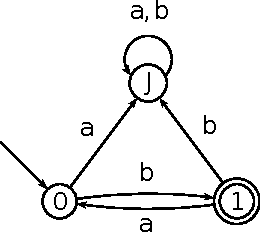
\includegraphics[width=0.7\linewidth]{automaten/Loesung2.pdf}
	\end{figure}
\end{frame}
}

\begin{frame}	
	\begin{block}{Was ihr nun wissen solltet}
		\begin{itemize}
			\item Was Automaten sind und wie sie funktionieren
			\item Spezialform: Endlicher Akzeptor!
			\item Ein Regelwerk: Reguläre Ausdrücke
		\end{itemize}
	\end{block}
	
	\begin{block}{Was nächstes Mal kommt}
		\begin{itemize}
			\item Rechtslineare Grammatiken
			\item Turingmaschinen -- mächtiger wird es nicht mehr!
		\end{itemize}
	\end{block}
\end{frame}


\xkcdframevert{1319}{Danke für eure Aufmerksamkeit! \smiley}{2.5}
%\lastframe{0.6}{30}{xkcd/automation_1319.png}{http://www.xkcd.com/1319}
%\xkcdframe{0.5}{30}{xkcd/houston_1438.png}{http://www.xkcd.com/1438}{Oh, hi mom. No, nothing important, just work.}



\slideThanks

\end{document}